% \documentclass{cumcmthesis}
\documentclass[withoutpreface,bwprint]{cumcmthesis} %去掉封面与编号页,电子版提交的时候使用。


\usepackage[framemethod=TikZ]{mdframed}
\usepackage{url}   % 网页链接
\usepackage{subcaption} % 子标题
\title{全国大学生数学建模竞赛编写的 \LaTeX{} 模板}
\tihao{A}
\baominghao{}
\schoolname{东南大学}
\membera{顾晋宁}
\memberb{徐睿正}
\memberc{尹卓凡}
\supervisor{}
\yearinput{2025}
\monthinput{08}
\dayinput{02}

\begin{document}

    \maketitle
    \begin{abstract}

        \keywords{\TeX{}\quad  图片\quad   表格\quad  公式}
    \end{abstract}

    \section{问题重述}
    \section{模型假设}
    \section{符号说明}
    \section{模型求解}
    \subsection{着陆准备轨道的建模}
    当嫦娥三号在着陆准备轨道上运动时,主要受到月球对其的引力;
    而其它天体的引力及耗散力极其微弱,可以忽略不计。
    因此,将运动过程简化为飞行器与月球的两体运动。
    在月球系下,飞行器围绕月球做椭圆轨道运动,
    其运动轨迹如图\ref{fig:tuo_yuan_gui_dao}所示。
    \begin{figure}[!h]
        \centering
        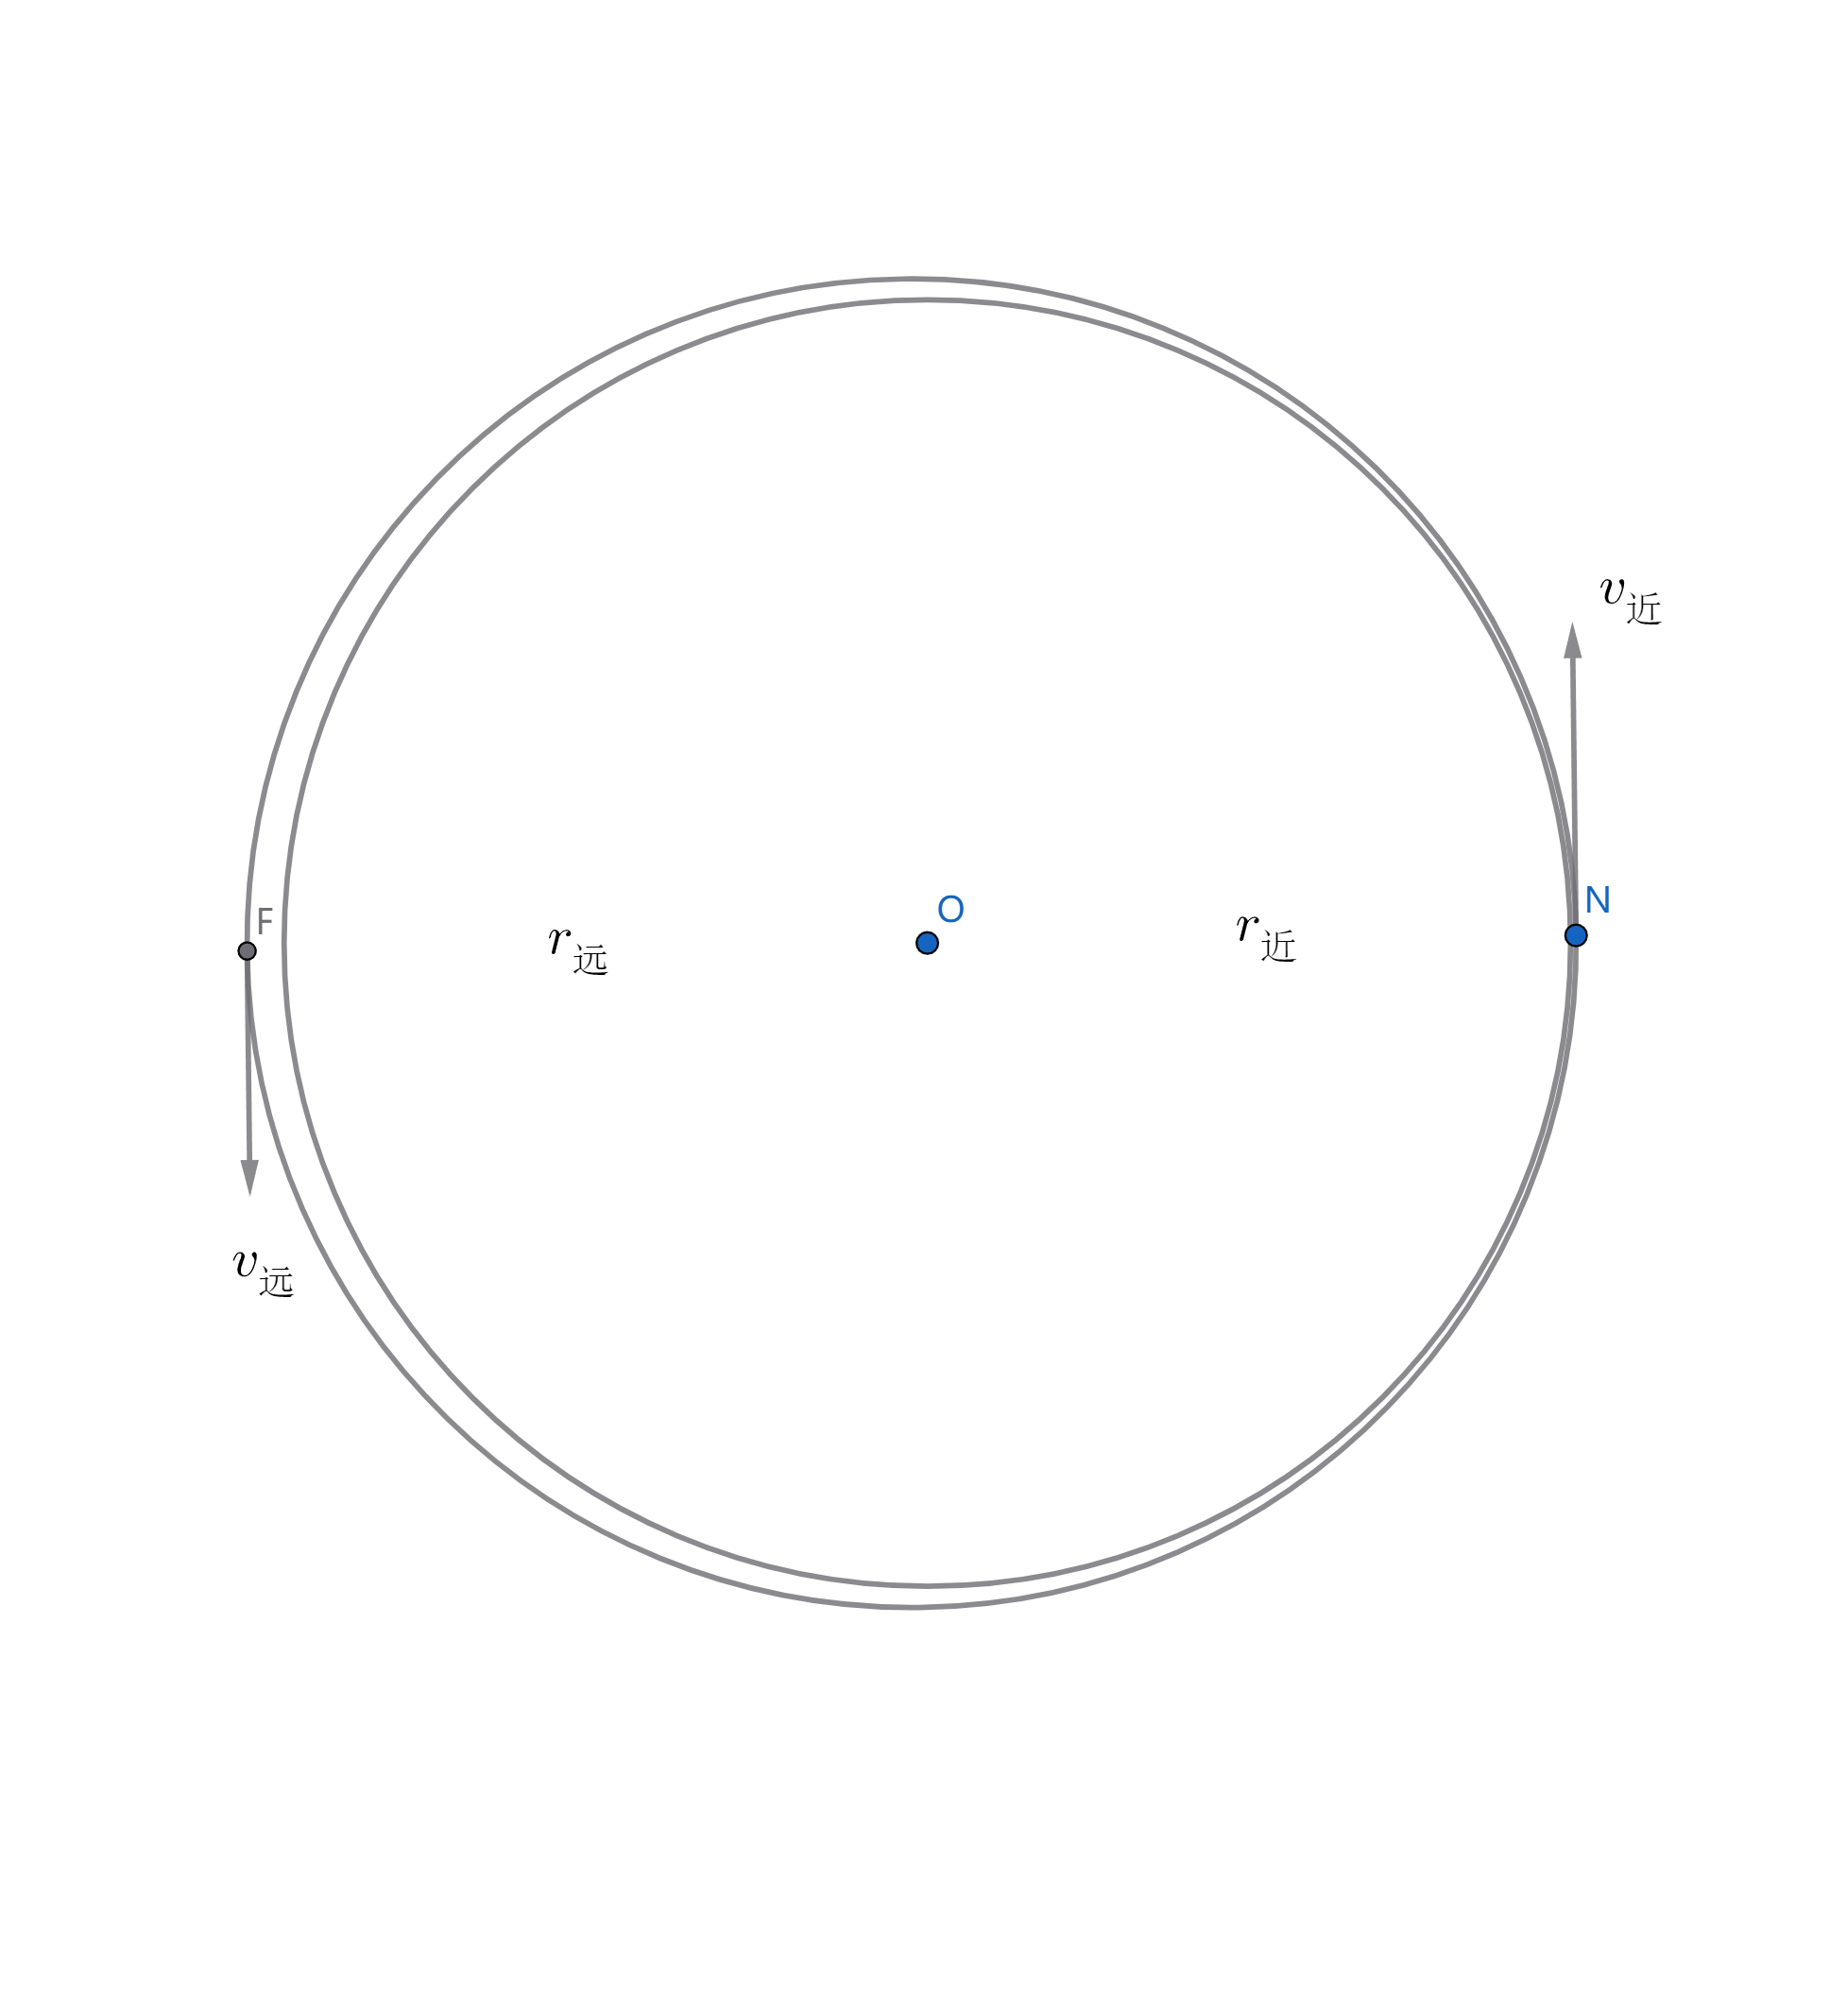
\includegraphics[width=.6\textwidth]{椭圆轨道}
        \caption{着陆准备轨道示意图}
        \label{fig:tuo_yuan_gui_dao}
    \end{figure}


    由角动量守恒定律与能量守恒定律可得
    \begin{equation}
        \begin{cases}
            m_0 v_Nr_N = m_0v_Fr_F \\
            \frac{1}{2} m_0 v_N^2 - \frac{GMm_0}{r_N} = \frac{1}{2} m_0 v_F^2 - \frac{GMm_0}{r_F}
        \end{cases}
    \end{equation}
    故
    \begin{equation}
        v_F = \frac{r_N}{r_F} v_N
        \label{eq:v_eq}
    \end{equation}
    \begin{equation*}
        v_N^2 - v_F^2 = 2GM(\frac{1}{r_N} - \frac{1}{r_F})
    \end{equation*}
    将(\ref{eq:v_eq})式代入得
    \begin{equation*}
        (1 - \frac{r_N^2}{r_F^2})v_N^2 = 2GM(\frac{1}{r_N} - \frac{1}{r_F})
    \end{equation*}
    因此
    \begin{equation}
        \boxed{
            v_N = \sqrt{\frac{2GMr_F}{r_N(r_N + r_F)}}
        }
    \end{equation}
    \subsection{主减速段轨道的建模}
    当飞行器到达近月点$N$时,其将转轨进入主减速段轨道。
    由题意可知,该段轨道的几何形状为抛物线。
    因此,飞行器在该段内具有恒定的受力。
    即
    \begin{equation}
        m\vec{g} + \vec{T} \equiv \vec{C}
        \label{eq:heng_li}
    \end{equation}


    而轨道初速度应与近月点相同,即
    \[
        \vec{v}_0 = \vec{v}_N
    \]
    记近月点的速率为$v_0$,故$\| \vec{v}_N \| = v_0$


    此外,题目还要求了主减速末端的速率$v_1$为一确定值。


    综上,轨道形状大致如图\ref{fig:jian_su_gui_dao}所示。
    \begin{figure}[!h]
        \centering
        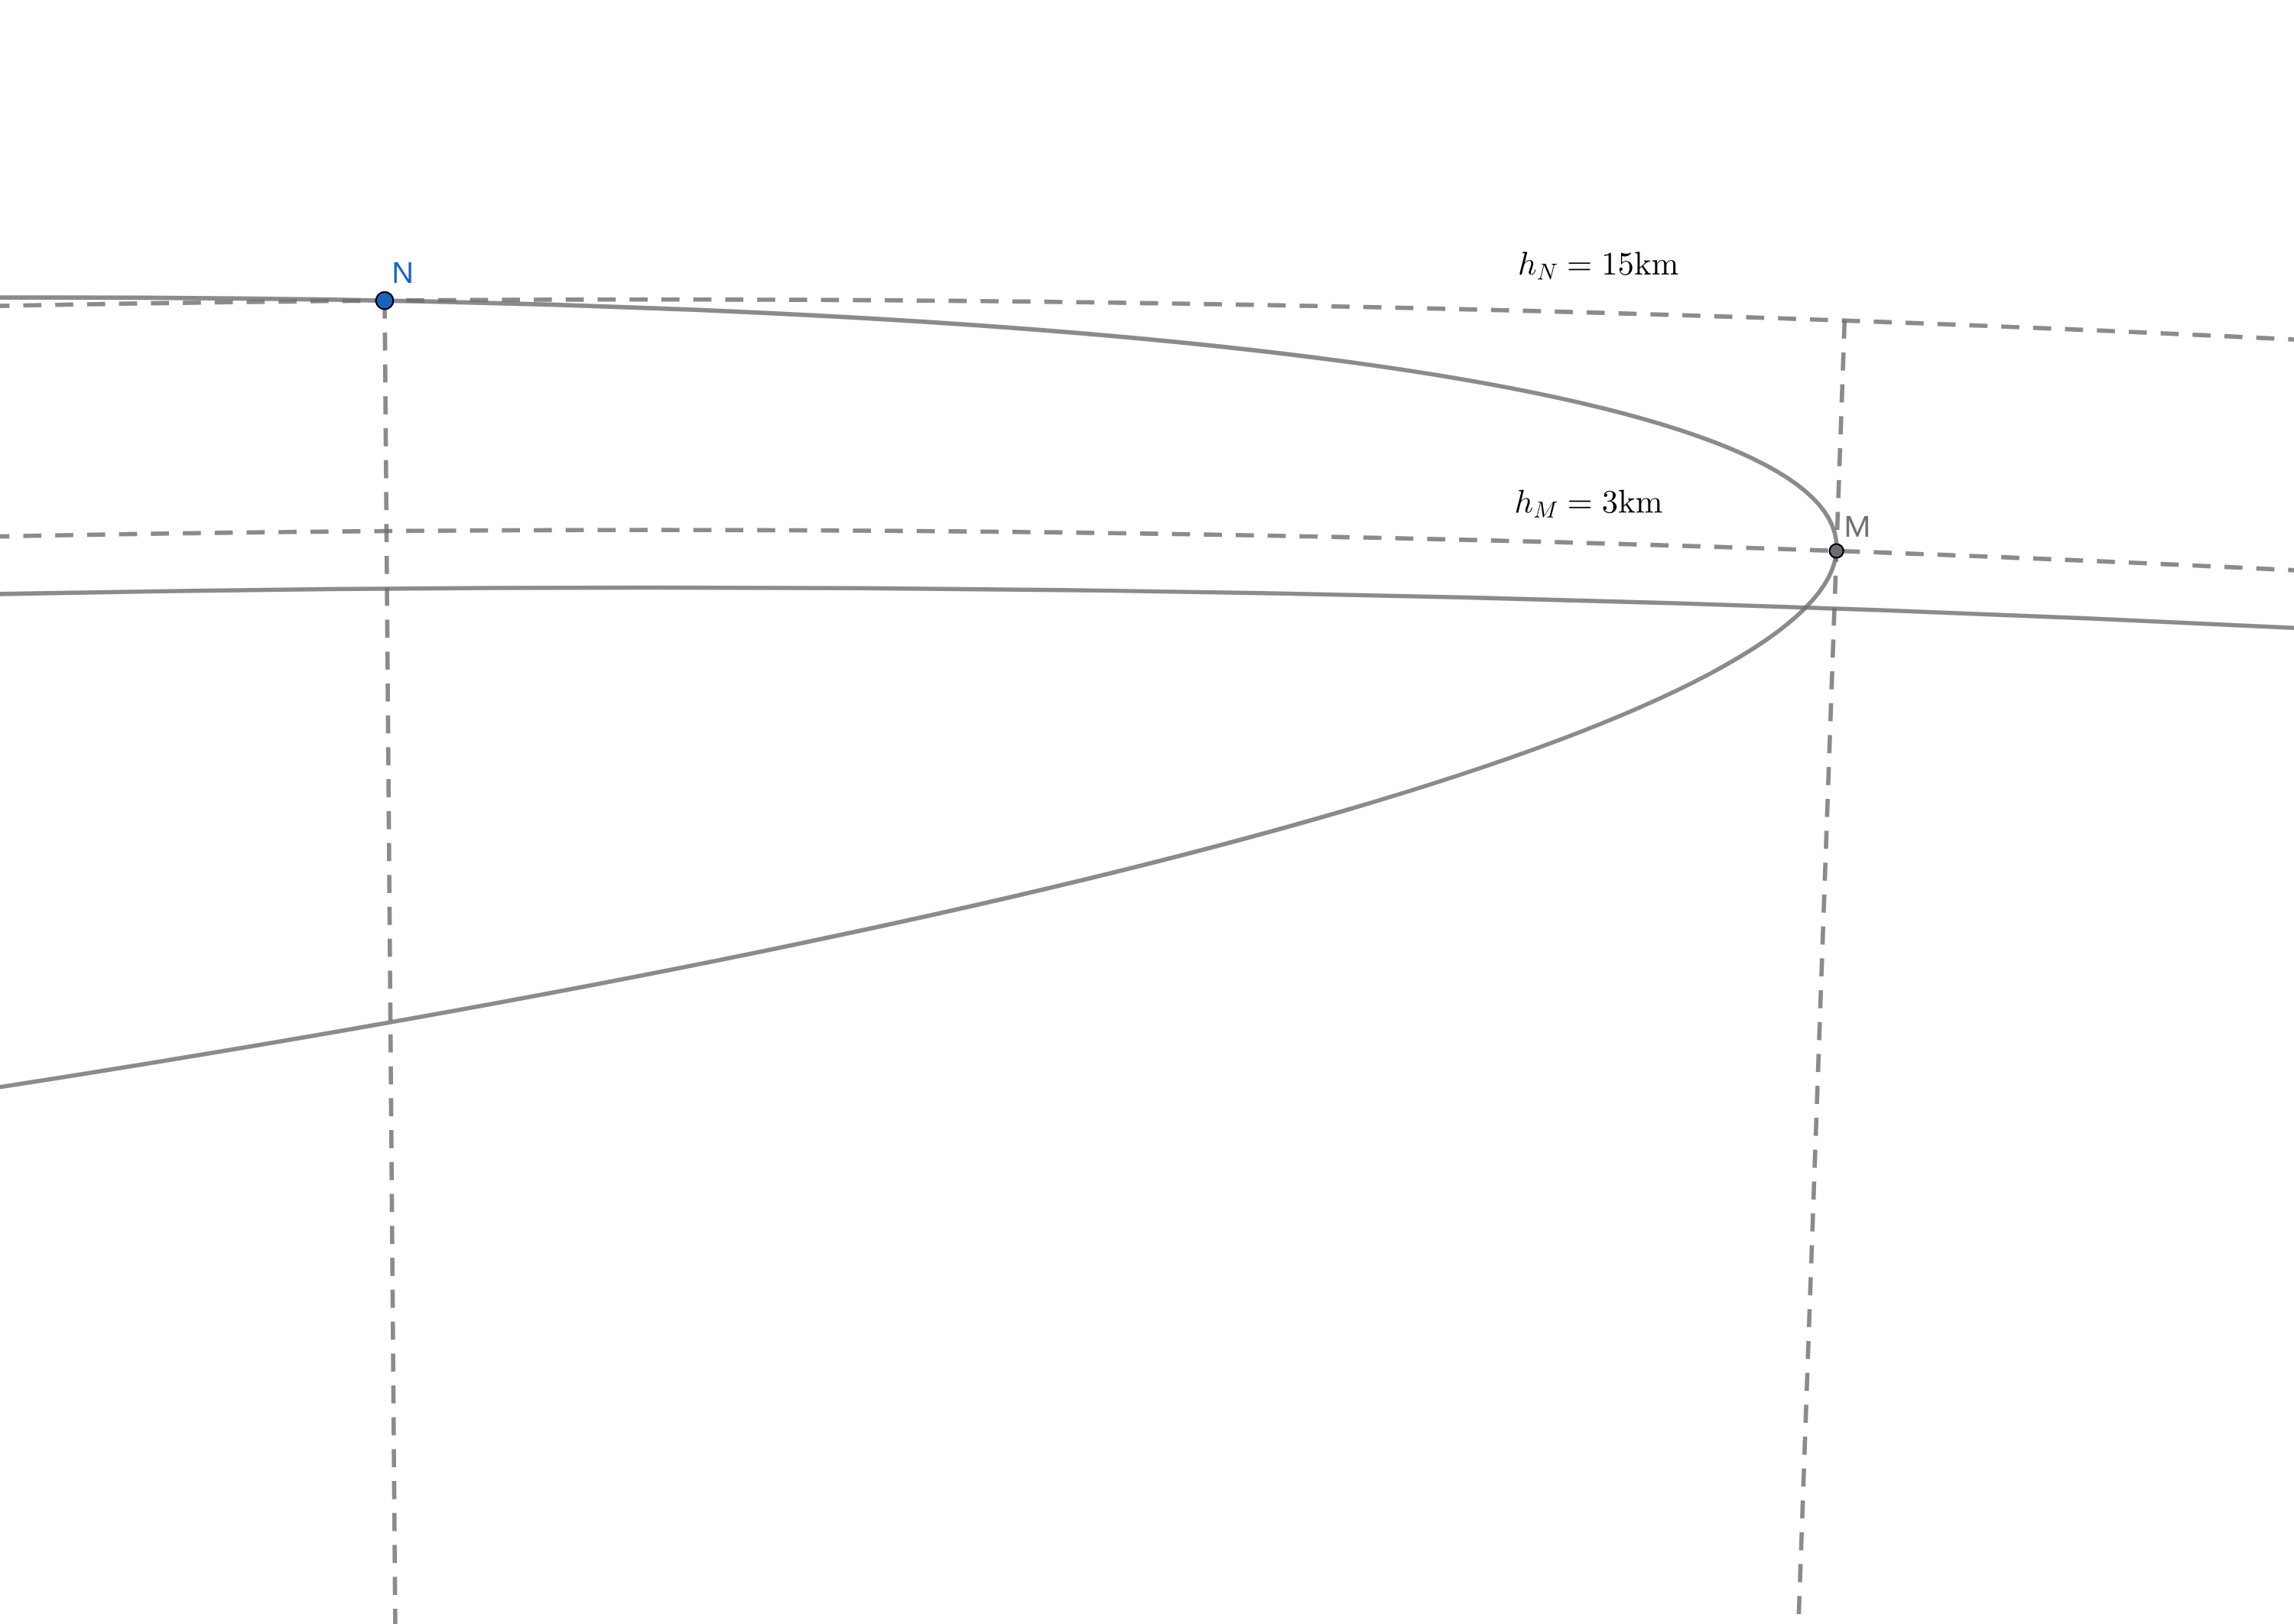
\includegraphics[width=.6\textwidth]{减速轨道}
        \caption{主减速段轨道示意图}
        \label{fig:jian_su_gui_dao}
    \end{figure}

    
    飞行器在该轨道内的运动过程时间较短,
    在球面方向内的运动距离相对月球半径较小。
    因此,可以将该过程近似至一直角坐标系内,
    竖直向下记为x轴正方向,球面方向记作y轴,如图\ref{fig:zhu_jian_su_duan_jian_xi}所示。
    \begin{figure}[!h]
        \centering
        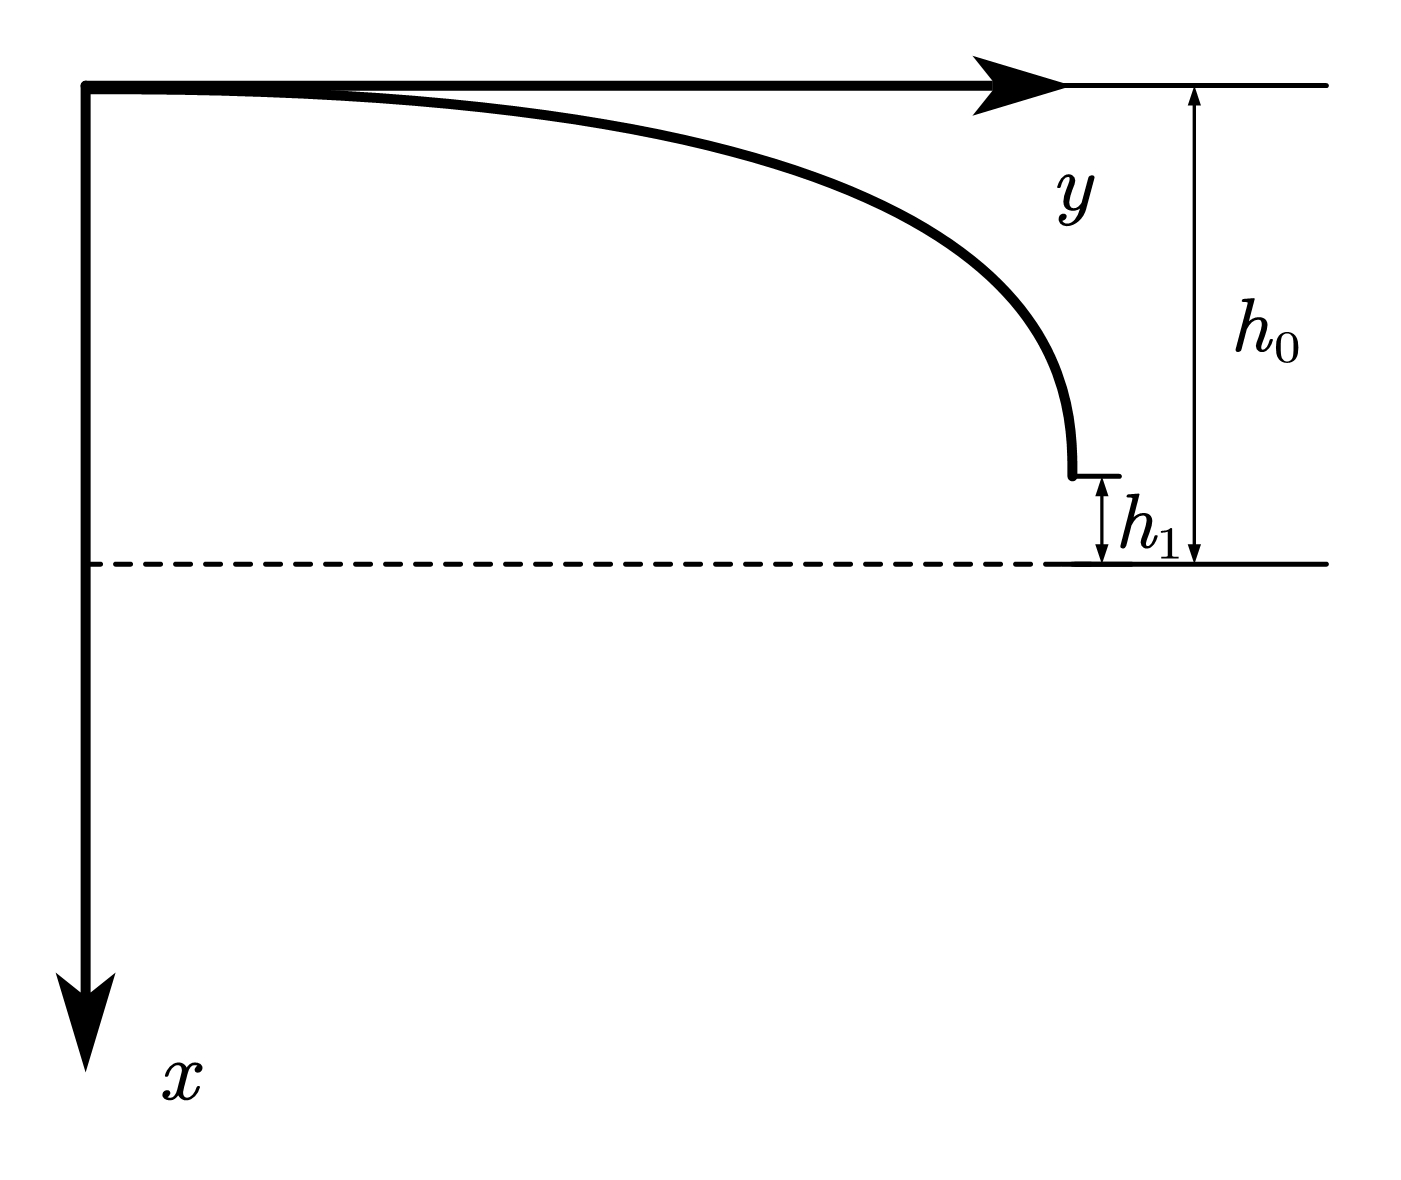
\includegraphics[width=.6\textwidth]{主减速段建系}
        \caption{主减速段在直角坐标系中的近似}
        \label{fig:zhu_jian_su_duan_jian_xi}
    \end{figure}


    此外,由于该过程中,距月心的距离变化$\Delta r$相对月球半径$R$的相对变化较小,
    故可以将重力加速度近似为一常量,其值取高度中值处的重力加速度$g$。
    此时,由恒力条件(\ref{eq:heng_li})式进一步分析,知$T$近似为一恒力。
    设$T$在$x,y$轴上的分量分别为$T_x, T_y$。
    

    该阶段飞行器的受力情况,如图\ref{fig:zhu_jian_su_shou_li}所示。
    \begin{figure}[!h]
        \centering
        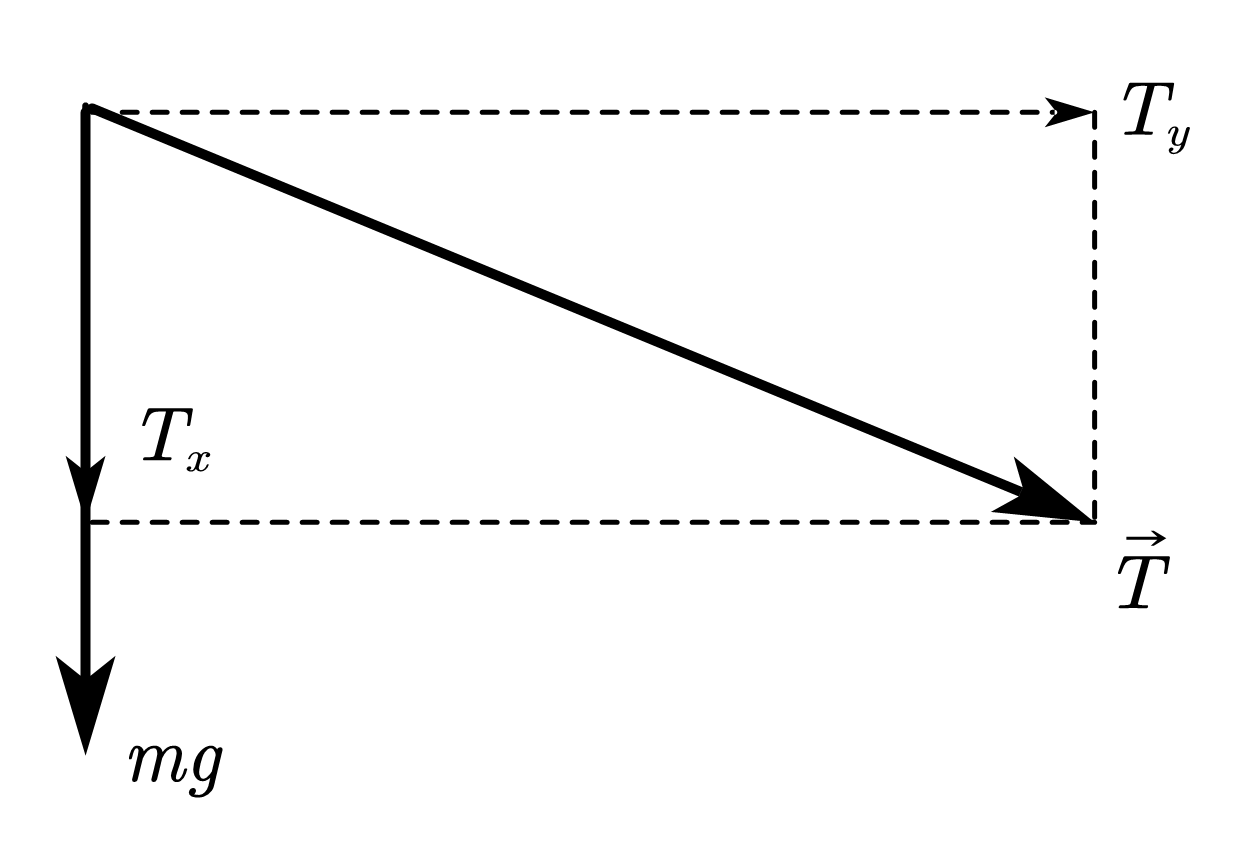
\includegraphics[width=.6\textwidth]{主减速受力}
        \caption{飞行器在主减速段的受力情况}
        \label{fig:zhu_jian_su_shou_li}
    \end{figure}


    因此,可以列得牛顿第二定律
    \begin{equation}
        \begin{cases}
            T_x + mg = m a_x \\
            T_y = m a_y
            \label{eq:niu_er}
        \end{cases}
    \end{equation}
    同时,满足比冲公式
    \begin{equation*}
        T = v_e |\dot{m}|
    \end{equation*}
    设质量减少的速率为$v_m$,因此
    \begin{equation}
        \boxed{
            v_m = |\dot{m}| = \frac{T}{v_e} = \frac{\sqrt{T_x^2 + T_y^2}}{v_e}
        }
    \end{equation}
    则质量关于时间的函数$m(t)$满足
    \begin{equation}
        m(t) = m_0 - v_m t
        \label{eq:m_t}
    \end{equation}
    将(\ref{eq:m_t})式代入(\ref{eq:niu_er})式,整理后得
    \begin{equation}
        \begin{cases}
            \ddot{x} = g + \frac{T_x}{m_0 - v_m t} \\
            \ddot{y} = \frac{T_y}{m_0 - v_m t}
        \end{cases}
    \end{equation}
    两边同时积分
    \begin{equation*}
        \begin{cases}
            \dot{x} = gt - \frac{T_x}{v_m}\ln(m_0 - v_m t) + C_1 \\
            \dot{y} = -\frac{T_y}{v_m}\ln(m_0 - v_m t) + C_2
        \end{cases}
    \end{equation*}
    代入初值条件
    \begin{equation*}
        \begin{cases}
            v_{0,x} = 0 \\
            v_{0,y} = v_0
        \end{cases}
    \end{equation*}
    解得
    \begin{equation*}
        \begin{cases}
            C_1 = \frac{T_x}{v_m}\ln m_0\\
            C_2 = v_0 + \frac{T_y}{v_m}\ln m_0
        \end{cases}
    \end{equation*}
    代回得
    \begin{equation}
        \begin{cases}
            \dot{x} = \frac{T_x}{v_m}\ln m_0 + gt - \frac{T_x}{v_m}\ln(m_0 - v_m t) \\
            \dot{y} = v_0 + \frac{T_y}{v_m}\ln m_0 - \frac{T_y}{v_m}\ln(m_0 - v_m t)
        \end{cases}
    \end{equation}
    取定积分得
    \begin{equation}
        \begin{cases}
            \Delta x = \frac{T_x}{v_m}\ln m_0 \cdot t + \frac{1}{2}gt^2
            - \frac{T_x}{v_m}((t - \frac{m_0}{v_m})\ln(m_0 - v_m t) - t) \\
            \Delta y = (v_0 + \frac{T_y}{v_m}\ln m_0) t
            - \frac{T_y}{v_m}((t - \frac{m_0}{v_m})\ln(m_0 - v_m t) - t)
        \end{cases}
    \end{equation}
    由于$\Delta x$为一定值,在给定的$T_x,T_y$条件下,可以算得时间$t$。
    由该$t$下的$\dot{x},\dot{y}$可以算得速率$v_1$,
    综合各个条件,可以得到优化模型
    \begin{equation}
        \begin{aligned}
            & \max m_1 = m_0 - v_m t \\
            s.t. &
            \begin{cases}
                T = \sqrt{T_x^2 + T_y^2} \\
                v_m = \frac{T}{v_e} \\
                \Delta x = \frac{T_x}{v_m}\ln m_0 \cdot t + \frac{1}{2}gt^2
                - \frac{T_x}{v_m}((t - \frac{m_0}{v_m})\ln(m_0 - v_m t) - t) \\
                \dot{x} = \frac{T_x}{v_m}\ln m_0 + gt - \frac{T_x}{v_m}\ln(m_0 - v_m t) \\
                \dot{y} = v_0 + \frac{T_y}{v_m}\ln m_0 - \frac{T_y}{v_m}\ln(m_0 - v_m t) \\
                v_1 = \sqrt{\dot{x}^2 + \dot{y}^2} \\
                1500 \le T \le 7500
            \end{cases}
        \end{aligned}
    \end{equation}
    设该NLP问题的解为$(T_x, T_y, t)$,由式
    \begin{equation*}
        \Delta y = (v_0 + \frac{T_y}{v_m}\ln m_0) t
        - \frac{T_y}{v_m}((t - \frac{m_0}{v_m})\ln(m_0 - v_m t) - t)
    \end{equation*}
    求得水平位移$\Delta y$。
    而通过水平位移以及轨道方向,可以得到近月点与目标着陆点的经纬度偏差。
    \subsection{月球经纬度偏差的求解}
    \subsection{快速调整阶段的建模}
    \subsection{粗避障段的建模}
    \subsection{精避障段的建模}
    \subsection{缓速下降段的建模}
    \subsection{}
    
    \section{模型检验}

    %参考文献
    \begin{thebibliography}{9}%宽度9
        \bibitem[1]{liuhaiyang2013latex}
        刘海洋.
        \newblock \LaTeX {}入门\allowbreak[J].
        \newblock 电子工业出版社, 北京, 2013.
        \bibitem[2]{mathematical-modeling}
        全国大学生数学建模竞赛论文格式规范 (2020 年 8 月 25 日修改).
        \bibitem{3} \url{https://www.latexstudio.net}
    \end{thebibliography}

    \newpage
    %附录
    \begin{appendices}
    \end{appendices}

\end{document} 